%Dette er en helt simpel skabelon, som kan bruges til at skrive almindelige 
%afleveringer i. Koden er bevidst lavet så ukompliceret som muligt,
%så dokumentet samtidigt kan bruges som en indgang til at læse LaTeX at kende.

%---------------------------------------------------------
%Dette er kun preample. Det behøver du ikke bekymre dig om. Går ned til der står "Start her". Eller til der hvor sidehovedet indstilles.
%---------------------------------------------------------
\documentclass[a4paper,12pt,oneside,article]{memoir}
% lidt marginer
\setlrmarginsandblock{3cm}{*}{1}
\setulmarginsandblock{3cm}{*}{1}
\setheadfoot{2cm}{\footskip}          % mere højde til sidehovedet
\checkandfixthelayout[nearest]

%Fjerner parindent ved nyt afsnit
\setlength{\parindent}{0pt}

% Standard dansk opsætning
\usepackage[utf8]{inputenc}   %æøå med utf8-encoding
\usepackage[danish]{babel}            % dansk opsætning
\renewcommand\danishhyphenmins{22}    % fikser en fejl i babel
\usepackage[T1]{fontenc} %fontencoding
\usepackage{lmodern} %sætter skrifttypen til Latin Modern
\usepackage{icomma}%Sørger for at man kan bruge komma som decimalseperator

% Matematiske symboler og fede tegn i ligninger
\usepackage{amsmath, amssymb, bm, mathtools, mathdots}

%Flere mulighder for understregning
\usepackage[normalem]{ulem}

% Tabeller og søjler
\usepackage{array, booktabs, tabularx}

% Figurer og farver
\usepackage{graphicx, caption, subfig}
\captionsetup{font=small,labelfont=bf}

%--------------------------------------------------------
%Her sættes sidehoved og sidefod. Skriv dit eget navn ind.
%--------------------------------------------------------

% Sidehoved og -fod
\makepagestyle{mypagestyle} %Min pagestyle med sidetal
\copypagestyle{mypagestyle}{empty}
\makeoddhead{mypagestyle}{Navn\\Klasse}{\quad}{\today\\Fag}
\makeheadrule{mypagestyle}{\textwidth}{\normalrulethickness}
\makeoddfoot{mypagestyle}{}{\thepage~af~\thelastpage}{} %Kræver to oversættelser

\pagestyle{mypagestyle} %aktiver ny sidehoved/-fod

%Punktopstilling
\usepackage{enumerate}

%Enheder
\usepackage[output-decimal-marker={,}]{siunitx}
\usepackage[dvipsnames,table,xcdraw]{xcolor}

%Talmængder
\newcommand{\R}{\mathbb{R}} %\R for reelle tal
\newcommand{\C}{\mathbb{C}} %\C for komplekse tal
\newcommand{\N}{\mathbb{N}} %\N for naturlige tal
\newcommand{\Z}{\mathbb{Z}} %\Z for hele tal
\newcommand{\Q}{\mathbb{Q}} %\Q for rationale tal
\newcommand{\dg}{^{\circ}}%Brug \dg til at indsætte gradtegn
\newcommand{\TT}[1]{\textcolor{NavyBlue}{{\textbf TT: #1 }}}
\newcommand{\CX}[1]{\textcolor{Cyan}{{\textbf CX: #1 }}}
%Til hyperlinks
\usepackage[hidelinks=true]{hyperref}

\begin{document}%Her begynder indholdet af dokumentet.

%-------------------------------------------
%START HER!
%-------------------------------------------

\chapter*{Aflevering X.X} %Stjernen i chapter fjerner nummereringen.

Dette er \emph{min} aflevering.

Her er den første ligning:\CX{fjsidfo}\TT{fsdfsfd}
\begin{equation}
	2x^2+4=6.\label{eq:ligning}
\end{equation}
Den hedder \eqref{eq:ligning}.

Jeg kan også skrive matematiske symboler direkte på en linje med at bruge dollartegn. Det har jeg gjort her: $f(x) = a_{n} x^{n} + a_{n-1}x^{n-1}+\cdots +a_{1}x + a_{0}$.

\section*{Matematiske tegn}
Her er en lille oversigt over nogle af de mest almindelige matematikkonstruktioner.

Gangetegn:
\begin{equation*}%En stjerne bruges til at angive en unummereret ligning.
	a\cdot b
\end{equation*}
Brøker:
\begin{equation*}
	\frac{a}{b}
\end{equation*}
Integraler:
\begin{equation*}
	\int_a^b f(x)\, dx. %Bemærk \, som giver lidt ekstra plads mellem f(x) og dx
\end{equation*}
Sumtegn:
\begin{equation*}
	\sum_{i=1}^n f(x_i) \Delta x
\end{equation*}
Grænseværdier:
\begin{equation*}
	\lim_{\Delta \to 0} \frac{f(x_0+\Delta x)-f(x_0)}{\Delta x}
\end{equation*}
Numerisk værdi:
\begin{equation*}
	\lvert -5 \rvert=5
\end{equation*}
Kvadratrod:
\begin{equation*}
	\sqrt{x+1}
\end{equation*}
Vektorer:
\begin{equation*}
	\vec{a} =\begin{pmatrix} 1\\2\\3 \end{pmatrix} \text{, } \widehat{\vec{a}} \text{ og } \overrightarrow{AB}
\end{equation*}
Mængder:
\begin{equation*}
	\{x \in \R \mid 2\leq x<5\} 
\end{equation*}
Gaffelforskrifter:
\begin{equation*}
	f(x) = \begin{cases}
	x^2 & \text{hvis } x>2,\\
	x-1 & \text{hvis } x\leq 2
	\end{cases}
\end{equation*}
Store parenteser:
\begin{equation*}
	\left(\frac{a}{b} \right)
\end{equation*}
Specielle tegn:
\begin{equation*}
	\pm \quad \infty \quad \leq \quad \geq \quad \circ \quad \in \quad \notin \quad \neq \quad \bullet \quad \Leftrightarrow \quad \Updownarrow \quad \times \quad \angle
\end{equation*}
Specielle funktioner:
\begin{equation*}
	\sin(x) \quad \cos(x) \quad \tan(x) \quad \ln(x) \quad \log(x) \quad \exp(x)
\end{equation*}

\section*{Formler med flere linjer}
Vi kan lave formler, der fylder flere linjer på denne måde:
\begin{align*}
	(a+b)^2 &= (a+b)(a+b)\\
	&= a^2+ab+ba+b^2\\
	&=a^2+2ab+b^2
\end{align*}
\section*{Punktopstillinger}
Her er en liste med tre punkter:
\begin{enumerate}[a)]
\item Første punkt
\item Andet punkt
\item Tredje punkt
\end{enumerate}

Her er en anden liste med en helt anden nummerering:
\begin{enumerate}[i)]
\item Første punkt
\item Andet punkt
\item Tredje punkt
\end{enumerate}

\section*{Tekst}
Det er let at skrive \textcolor{red}{farvet}, \textbf{fed} eller \textit{kursiv} tekst i \LaTeX. Det kan man sådan set også gøre i matematikmode\footnote{Her kommer bogstaverne dog som udgangspunkt i kursiv.}:
\begin{equation*}
	\textcolor{blue}{a^2}+\textrm{b}^2=\bm{c^2} \text{ eller } \uline{a+b}=\uuline{\SI{4,56e4}{kg.m^2.s^{-3}}{}}.
\end{equation*}
Det sidste eksempel gav også et tip til enheder og videnskabelig notation.

\section*{Figurer}

Det er ikke helt let at arbejde med figurer i \LaTeX, men man kan indsætte et centreret billede på denne måde:
\begin{center}
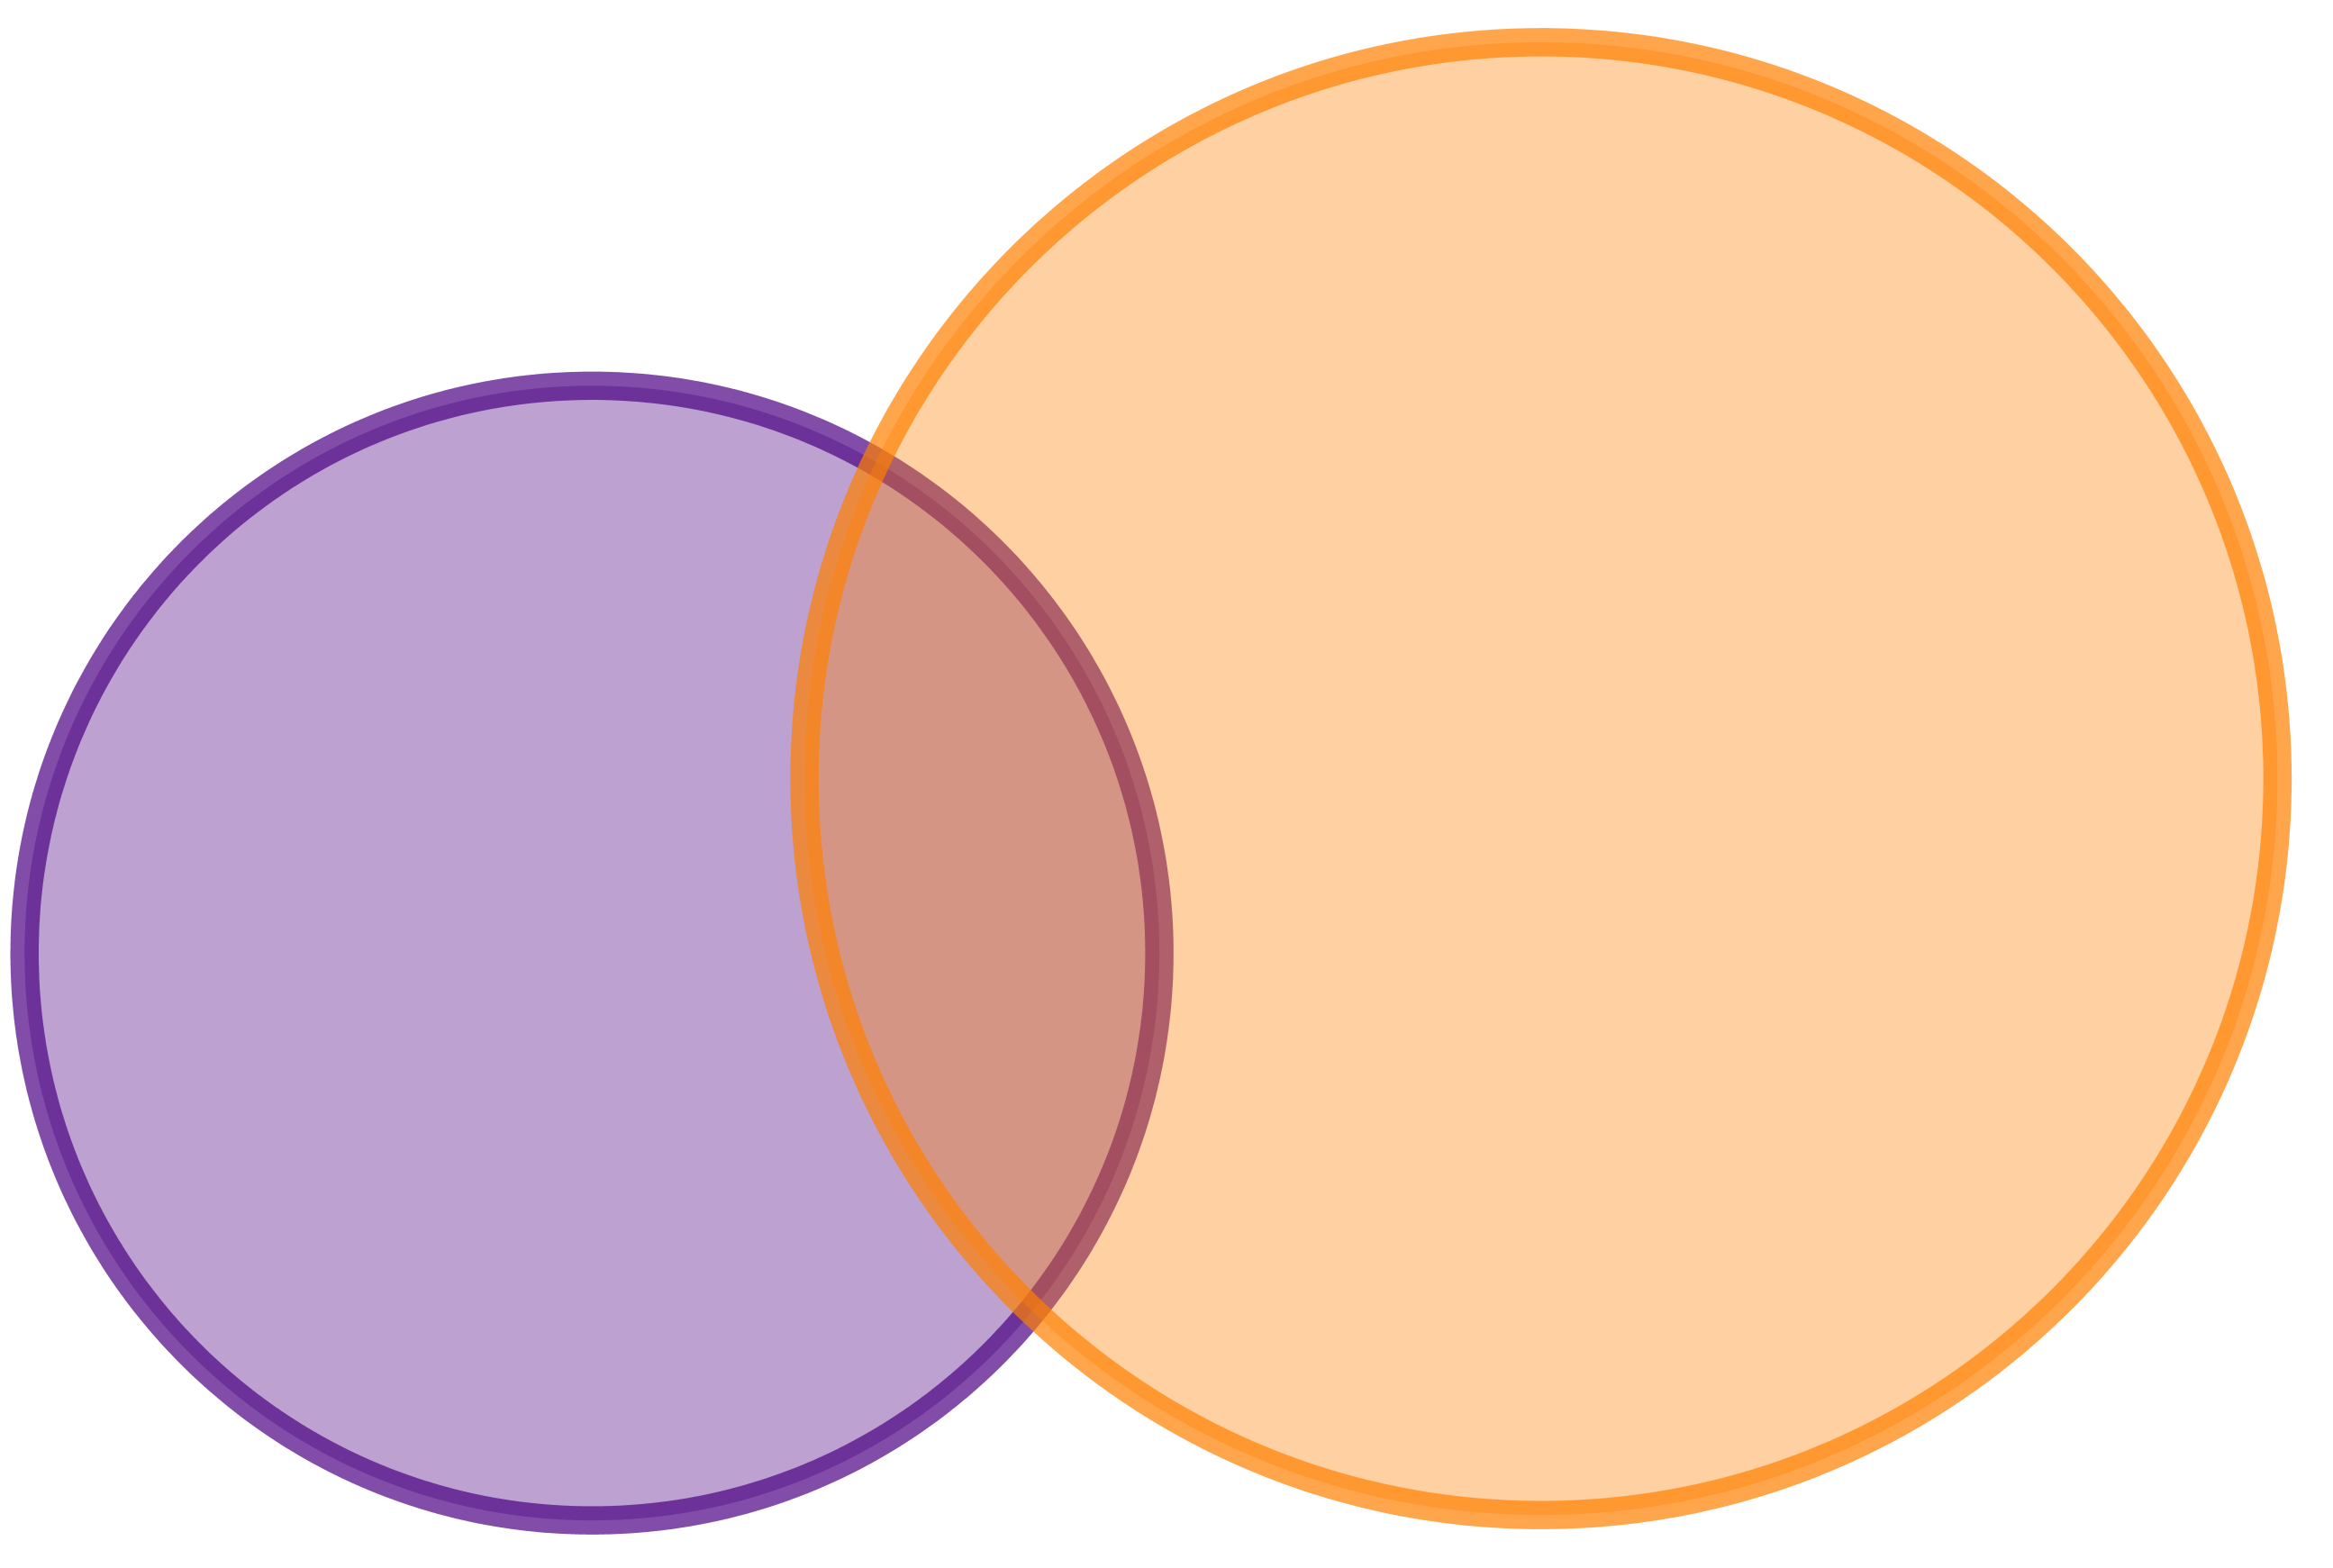
\includegraphics[width=4cm]{cirkler.png}
\captionof{figure}{Her er to cirkler.}\label{fig:smiley}
\end{center}
Billedet hedder figur \ref{fig:smiley}.

\chapter*{Yderligere læsning}
Hvis man er interesseret i at læse mere om \LaTeX, er der mange steder, hvor man kan hente mere hjælp. Den mest omfattende introduktion på dansk er nok Lars Madsens bog, som kan downloades her:
\begin{center}
	\url{http://math.au.dk/videnudveksling/latex/bog/}
\end{center}

%---------------------------------------------------------
%Dokumentet er slut.
%---------------------------------------------------------
\end{document}%Alt efter denne linje kommer ikke med i dokumentet.